\documentclass[a4paper,7pt,oneside]{book}

\usepackage{graphicx}
\usepackage{caption}
\usepackage{subcaption}
\usepackage{url}
\usepackage{color, colortbl} 	% to use colors in tables
\usepackage{tikz}
\usepackage{pgfplots}
\usepackage[a4paper]{geometry}
\usepackage{amsmath}

\newcommand\chap[1]{\chapter*{#1}\addcontentsline{toc}{chapter}{\protect\numberline{}#1}}
\definecolor{LightCyan}{rgb}{0.76, 0.92, 1}

\author{Zen Roberto}
\title{Language Understanding Systems - First Project Report}
\date{\today}

\begin{document}

% GOOD Report that includes:
% Data Analysis
% Evaluation
% Comparison of different:
% Feature Sets
% Tool Configurations

\begin{titlepage}
	\pagestyle{empty}

	\begin{center}
		{\bfseries\Large {\huge U}NIVERSITY OF {\huge T}RENTO}

		\vspace{0.2cm}

		{\large Department of Information Engineering and Computer Science}

		\vspace{0.5cm}

		\begin{center}
			
\includegraphics[width=0.3\textwidth]{res/unitn}
		\end{center}

		\vspace{2.5cm}

		{\Large \bfseries {{\huge L}ANGUAGE {\huge U}NDERSTANDING} {\huge S}YSTEMS}

		\vspace{0.5cm}

		{\Large \bfseries {FIRST PROJECT}}

		\vspace{1.5cm}
		
		{\large \textsc{Roberto Zen}}

		\vspace{1.0cm}
		
		{\today}

		\vspace{6.0cm}

		\small{The conducted work described in this report is currently released under the MIT license and it is available on \url{https://github.com/robzenn92/LUS}.}

		\vfill

	\end{center}

\end{titlepage}


% \tableofcontents

\newgeometry{top=32mm,bottom=32mm,left=32mm,right=32mm}

\chapter{Introduction and Data Analysis}

The report is structured as follows. In this chapter a data analysis of the given dataset is done. Chapter 2 describes how I used the \textit{FST} and \textit{GRM} tools for training and testing sequence labeling based on POS-Tagging. In addition, it shows the results of applying these tools with different Language Model (LM) parameters. As Chapter 2, Chapter 3 describes sequence labeling and results but using the \textit{CRF++} tool instead. Chapter 4 shows how text classification is made using \textit{Na\"{\i}ve Bayes}. The last section states the results and the conclusion of the conducted work.

The given data set is composed as follows.

\begin{table}[h!]
\small
	\begin{center}
	\begin{tabular}{|l|l|l|l|}
		\hline
		File name & Used for & Word count & Token count \\ \hline

		NLSPARQL.test.feats.txt	& FST & 0 & 0 \\ \hline
		NLSPARQL.train.feats.txt & FST & 0 & 0 \\ \hline
		
		NLSPARQL.test.data	& CFF++ & 7117 & 0 \\ \hline
		NLSPARQL.train.data	& CFF++ & 0 & 0 \\ \hline
		
		NLSPARQL.train.tok	& Naive Bayes & 0 & 0 \\ \hline
		NLSPARQL.train.utt.labels.txt & Naive Bayes & 0 & 0 \\ \hline
		NLSPARQL.test.tok	& Naive Bayes & 0 & 0 \\ \hline
		NLSPARQL.test.utt.labels.txt & Naive Bayes & 0 & 0 \\ \hline
		
	\end{tabular}
	\caption{Test results with FST.}
	\label{table:fst_results}
	\end{center}
\end{table}


\begin{figure}[h!]
  \centering
    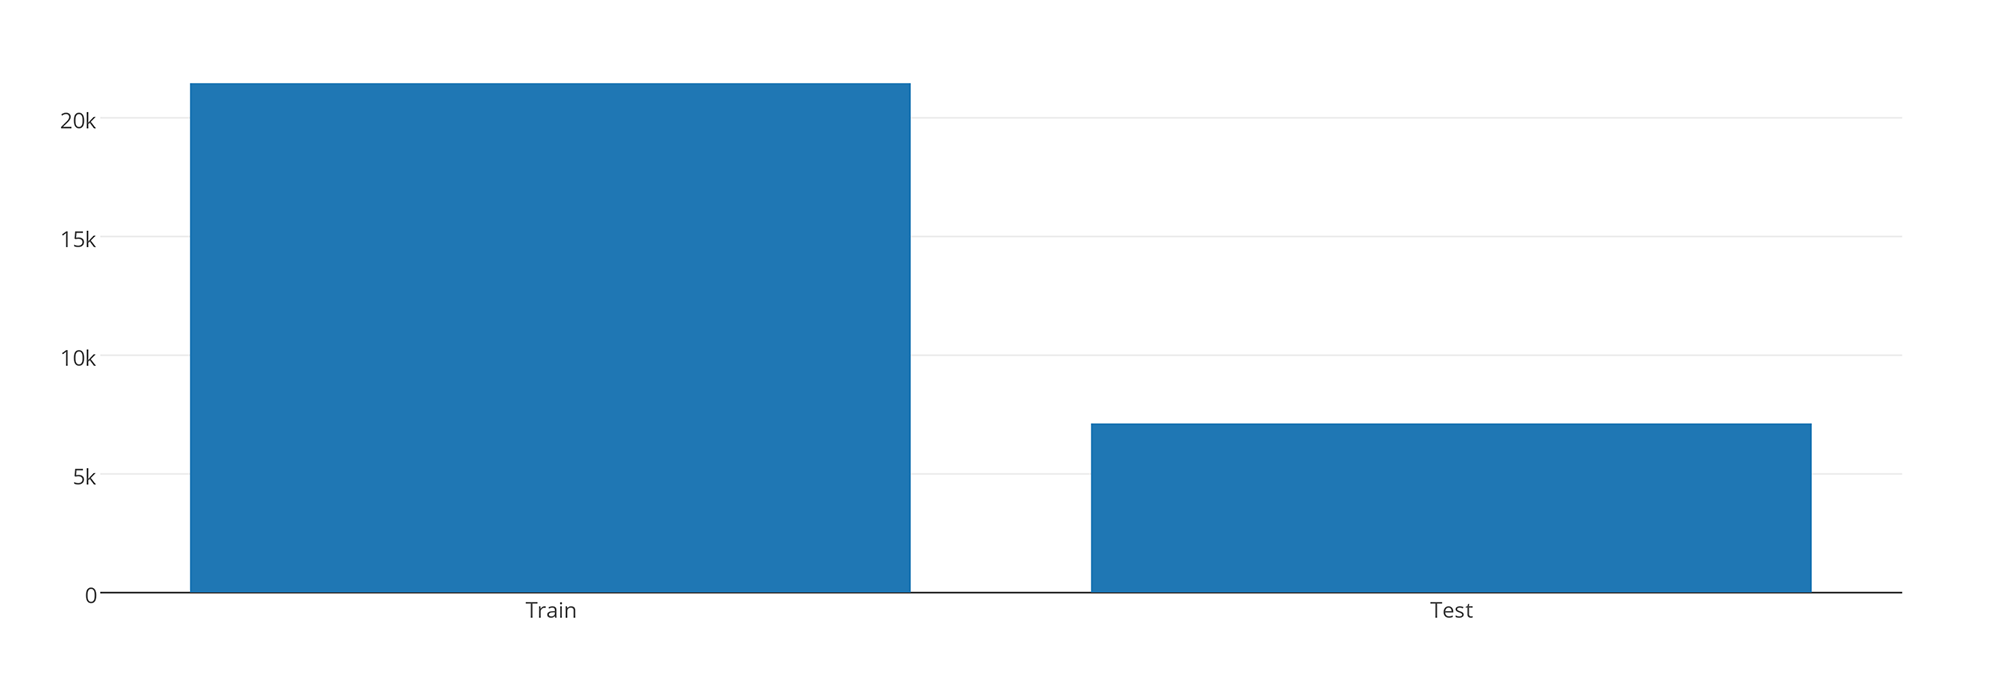
\includegraphics[scale=0.5]{res/crf_dataset_small}
    \caption{The word count for the train and the test dataset.}
    \label{fig:crf_dataset}
\end{figure}

\noindent
For each part of this work (FST, CRF, \textit{Na\"{\i}ve Bayes}), a tool named \textbf{CoNLL}\footnote{\url{https://github.com/tpeng/npchunker/blob/master/conlleval.pl}} has been used to evaluate the results of conducted tests. The level of parameters such as accuracy, precision and recall are used to compare LMs which might use different feature sets or tool configurations.

\chapter{Sequence labeling with FST}

The LM I trained and tested for this part is based on \textit{Finite State Transducers} (FST). In fact, it is based on a composition of them. For each sentence that belongs to the test file\footnote{\textbf{NLSPARQL.test.feats.txt}}, I built a FST in which each transition is labbeled with a pair word-word. Figure \ref{fig:fst_train_example} shows the FST built for the sentence ``who plays luke on star wars".

\begin{figure}[h!]
  \centering
    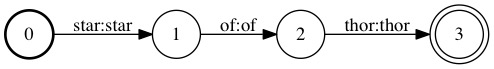
\includegraphics[scale=0.4]{res/fst_train_example}
    \caption{The FST built for a sentence that belongs to the train set.}
    \label{fig:fst_train_example}
\end{figure}

\noindent
Each of these FSTs is then composed with another one, in which there is only one final state and transitions that loop in it. Each transition is made by a pair word-tag and a weigth which is calculated as reported in the following expression. Note that unknown words has been considered as well.

\[ W_{ML}(w_i | tag_j) = \left\{ 
  \begin{array}{l l}
    - \log \left(\frac{C(w_i | tag_j)}{C(tag_j)}\right) & \quad \text{if $w_i$ is a knwon word}\\
    - \log \left(\frac{1}{|tagj|}\right) = - \log \left(\frac{1}{49}\right) & \quad \text{if $w_i$ is an unknown word}
  \end{array} \right.
 \]
\vspace{0.1cm}

\noindent
For the train part, I tried different approaches. First of all, I created the lexicon file based on the words, the tokens and also the lemmas written in the train file. Afterwards, I trained the model first considering lemmas as knonw words and then not. I got better results testing the model in the second case. Then, I experimented various train models with different ngramcount complexity orders. I started from the option \textbf{--order} set to value 1 and then I sequentially incremented it up to 6. Finally I tested the LM for each model configuration. Results for each parameter are shown in Table \ref{table:fst_results}.

\begin{table}[h!]
\small
	\begin{center}
	\begin{tabular}{|l|l|l|l|l|}
		\cline{2-5}
		\multicolumn{1}{r|}{} & accuracy & precision & recall & FB1 \\ \hline
		simple unigram-based POS-Tagger & 84.91\%  & 83.20\% &  84.61\% & 83.90 \\ \hline
		ngramcount --order=1 & 91.26\% & 89.97\% & 89.58\% & 89.77 \\ \hline
		ngramcount --order=2 & 93.37\% & 91.98\% & 92.45\% & 92.21 \\ \hline
		ngramcount --order=3 & 93.80\% & 92.51\% & 93.04\% & 92.77 \\ \hline \rowcolor{LightCyan}
		ngramcount --order=4 & 94.13\% & 92.87\% & 93.29\% & 93.08 \\ \hline
		ngramcount --order=5 & 93.97\% & 92.65\% & 93.07\% & 92.86 \\ \hline
		ngramcount --order=6 & 93.97\% & 92.77\% & 93.01\% & 92.89 \\ \hline
	\end{tabular}
	\caption{Test results with FST.}
	\label{table:fst_results}
	\end{center}
\end{table}

\noindent
The values shown in Table \ref{table:fst_results} are depicted in Figure \ref{fig:fst_ngram_count_levels}. As can be seen, although from order 1 to 2 there is a huge gap, the level of accuracy and of all the other parameters seems to stabilize with an ngram count value greather equal than 3. Hence, when the model counts trigrams or bigger n-grams. This mean that training the model with bigrams rather than unigrams we reach a very high level of accuracy. However, we reached better results training the LM with trigrams and ngrams.

\begin{figure}[h]
  \centering
    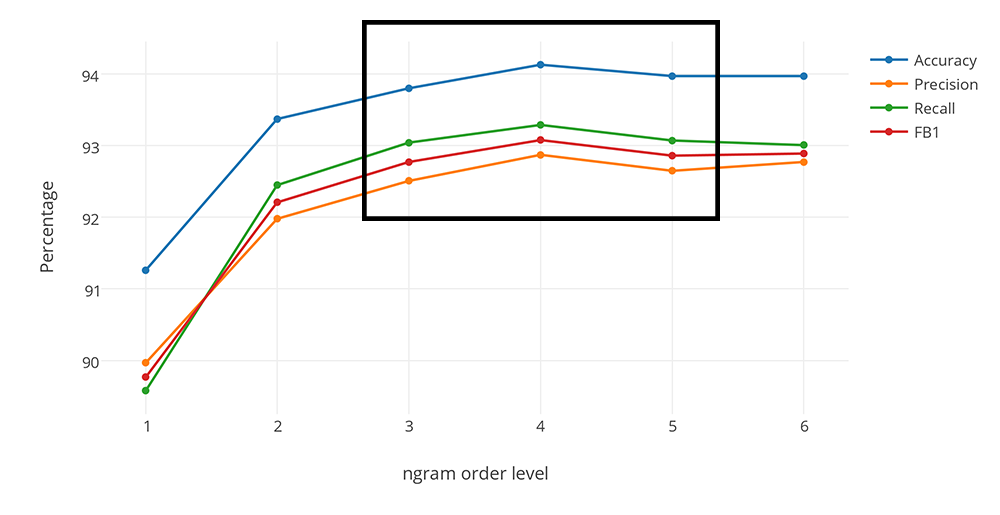
\includegraphics[scale=1.2]{res/fst_ngram_count_levels_small_rect}
    \caption{Test results of the LM which use different ngram count order's levels.}
    \label{fig:fst_ngram_count_levels}
\end{figure}

\noindent
As conclusion, I think that training the LM using trigrams rather than complex n-grams is the best choice because we reached a high precision and accuracy level maintaining the training task as simple as possible.

\chapter{Sequence labeling with CRF++}

I used Conditional Random Fields (CRFs) for the sequence labeling starting from training a LM based on the train file\footnote{NLSPARQL.train.data} written in IOB notation. I trained the LM using various template definition, however only four templates which gave me better results are written in Table \ref{table:crf_templates}.

These templates differ one each other for relevant reasons: the first two use only unigrams while the others use both unigrams and bigrams. Template A is the simplest one, its window has size 5 while Template B's window has size 7. Template C is defined as 7 unigrams and 3 bigrams while template D is the most complicated one, because it is made of 5 unigrams and 4 bigrams.

\begin{table}[!htb]
    \begin{minipage}[b]{.21\linewidth}
      \caption{Temp. A}
      \centering
        \begin{tabular}{|l|}
		\hline
		U00:\%x[-2,0] \hspace{2em} \\
		U01:\%x[-1,0] \\
		U02:\%x[0,0] \\
		U03:\%x[1,0] \\
		U04:\%x[2,0] \\ \hline
		\end{tabular}
    \end{minipage}
    \quad
    \begin{minipage}[b]{.21\linewidth}
      \caption{Temp. B}
      \centering
        \begin{tabular}{|l|}
		\hline
		U00:\%x[-3,0] \hspace{1.9em} \\
		U01:\%x[-2,0] \\
		U02:\%x[-1,0] \\
		U03:\%x[0,0] \\
		U04:\%x[1,0] \\
		U05:\%x[2,0] \\
		U06:\%x[3,0] \\ \hline
		\end{tabular}
    \end{minipage}
    \quad
    \begin{minipage}[b]{.24\linewidth}
      \caption{Temp. C}
      \centering
        \begin{tabular}{|l|}
		\hline
		U00:\%x[-2,0] \hspace{1.9em} \\
		U01:\%x[-1,0] \\
		U02:\%x[0,0] \\
		U03:\%x[1,0] \\
		U04:\%x[2,0] \\
		U05:\%x[-1,0]/\%x[0,0] \\
		U06:\%x[0,0]/\%x[1,0] \\
		U07:\%x[1,0]/\%x[2,0] \\
		B00:\%x[-1,0] \\
		B01:\%x[0,0] \\
		B02:\%x[1,0] \\ \hline
		\end{tabular}
	\end{minipage}
	\quad
    \begin{minipage}[b]{.22\linewidth}
      \caption{Temp. D}
      \centering
        \begin{tabular}{|l|}
		\hline
		U00:\%x[-1,0] \hspace{1.9em} \\
		U01:\%x[0,0] \\
		U02:\%x[1,0] \\
		U03:\%x[-1,0]/\%x[0,0] \\
		U04:\%x[0,0]/\%x[1,0] \\
		U05:\%x[1,0]/\%x[2,0] \\
		B00:\%x[-2,0] \\
		B01:\%x[-1,0] \\
		B02:\%x[0,0] \\
		B03:\%x[1,0] \\
		B04:\%x[2,0] \\ \hline
		\end{tabular}
    \end{minipage}
    \caption{CRF Templates.}
    \label{table:crf_templates}
\end{table}

\noindent
Regarding tool parameters, I trained the LM with different levels of \textit{cut-off} using the \textit{crf\_learn} command with the -f option value set initially to 1, then 2 and finally 3. As can be seen in Table \ref{table:crf_results}, I got better results with the default value\footnote{As written in \url{http://taku910.github.io/crfpp}, the default cut-off value for crf\_learn is 1.}.

\begin{table}[h!]
\small
	\begin{center}
	\begin{tabular}{|l|l|l|l|l|l|}
		\cline{2-6}
		\multicolumn{1}{r|}{} & accuracy & precision & recall & FB1 & \#features \\ \hline
		Template A & 93.59\% & 74.74\% & 73.24\% & 73.98 & 304958 \\ \hline
		Template B & 93.48\% & 78.01\% & 74.15\% & 76.03 & 399873 \\ \hline
		Template C & 94.28\% & 84.79\% & 78.19\% & 81.35 & 8804873 \\ \hline \rowcolor{LightCyan}
		Template D & 94.34\% & 86.13\% & 78.55\% & 82.17 & 12974573 \\ \hline
	\end{tabular}
	\caption{Test results with CRF++.}
	\label{table:crf_results}
	\end{center}
\end{table}

As can be seen in Figure \ref{fig:crf_exp_num_features}, there is an exponential increase of the number of feaures with respect to the level of precision. As a consequence, to the best of my knowledge it is often more convenient to use simple models as the one defined by the Template C.

\begin{figure}[h]
  \centering
    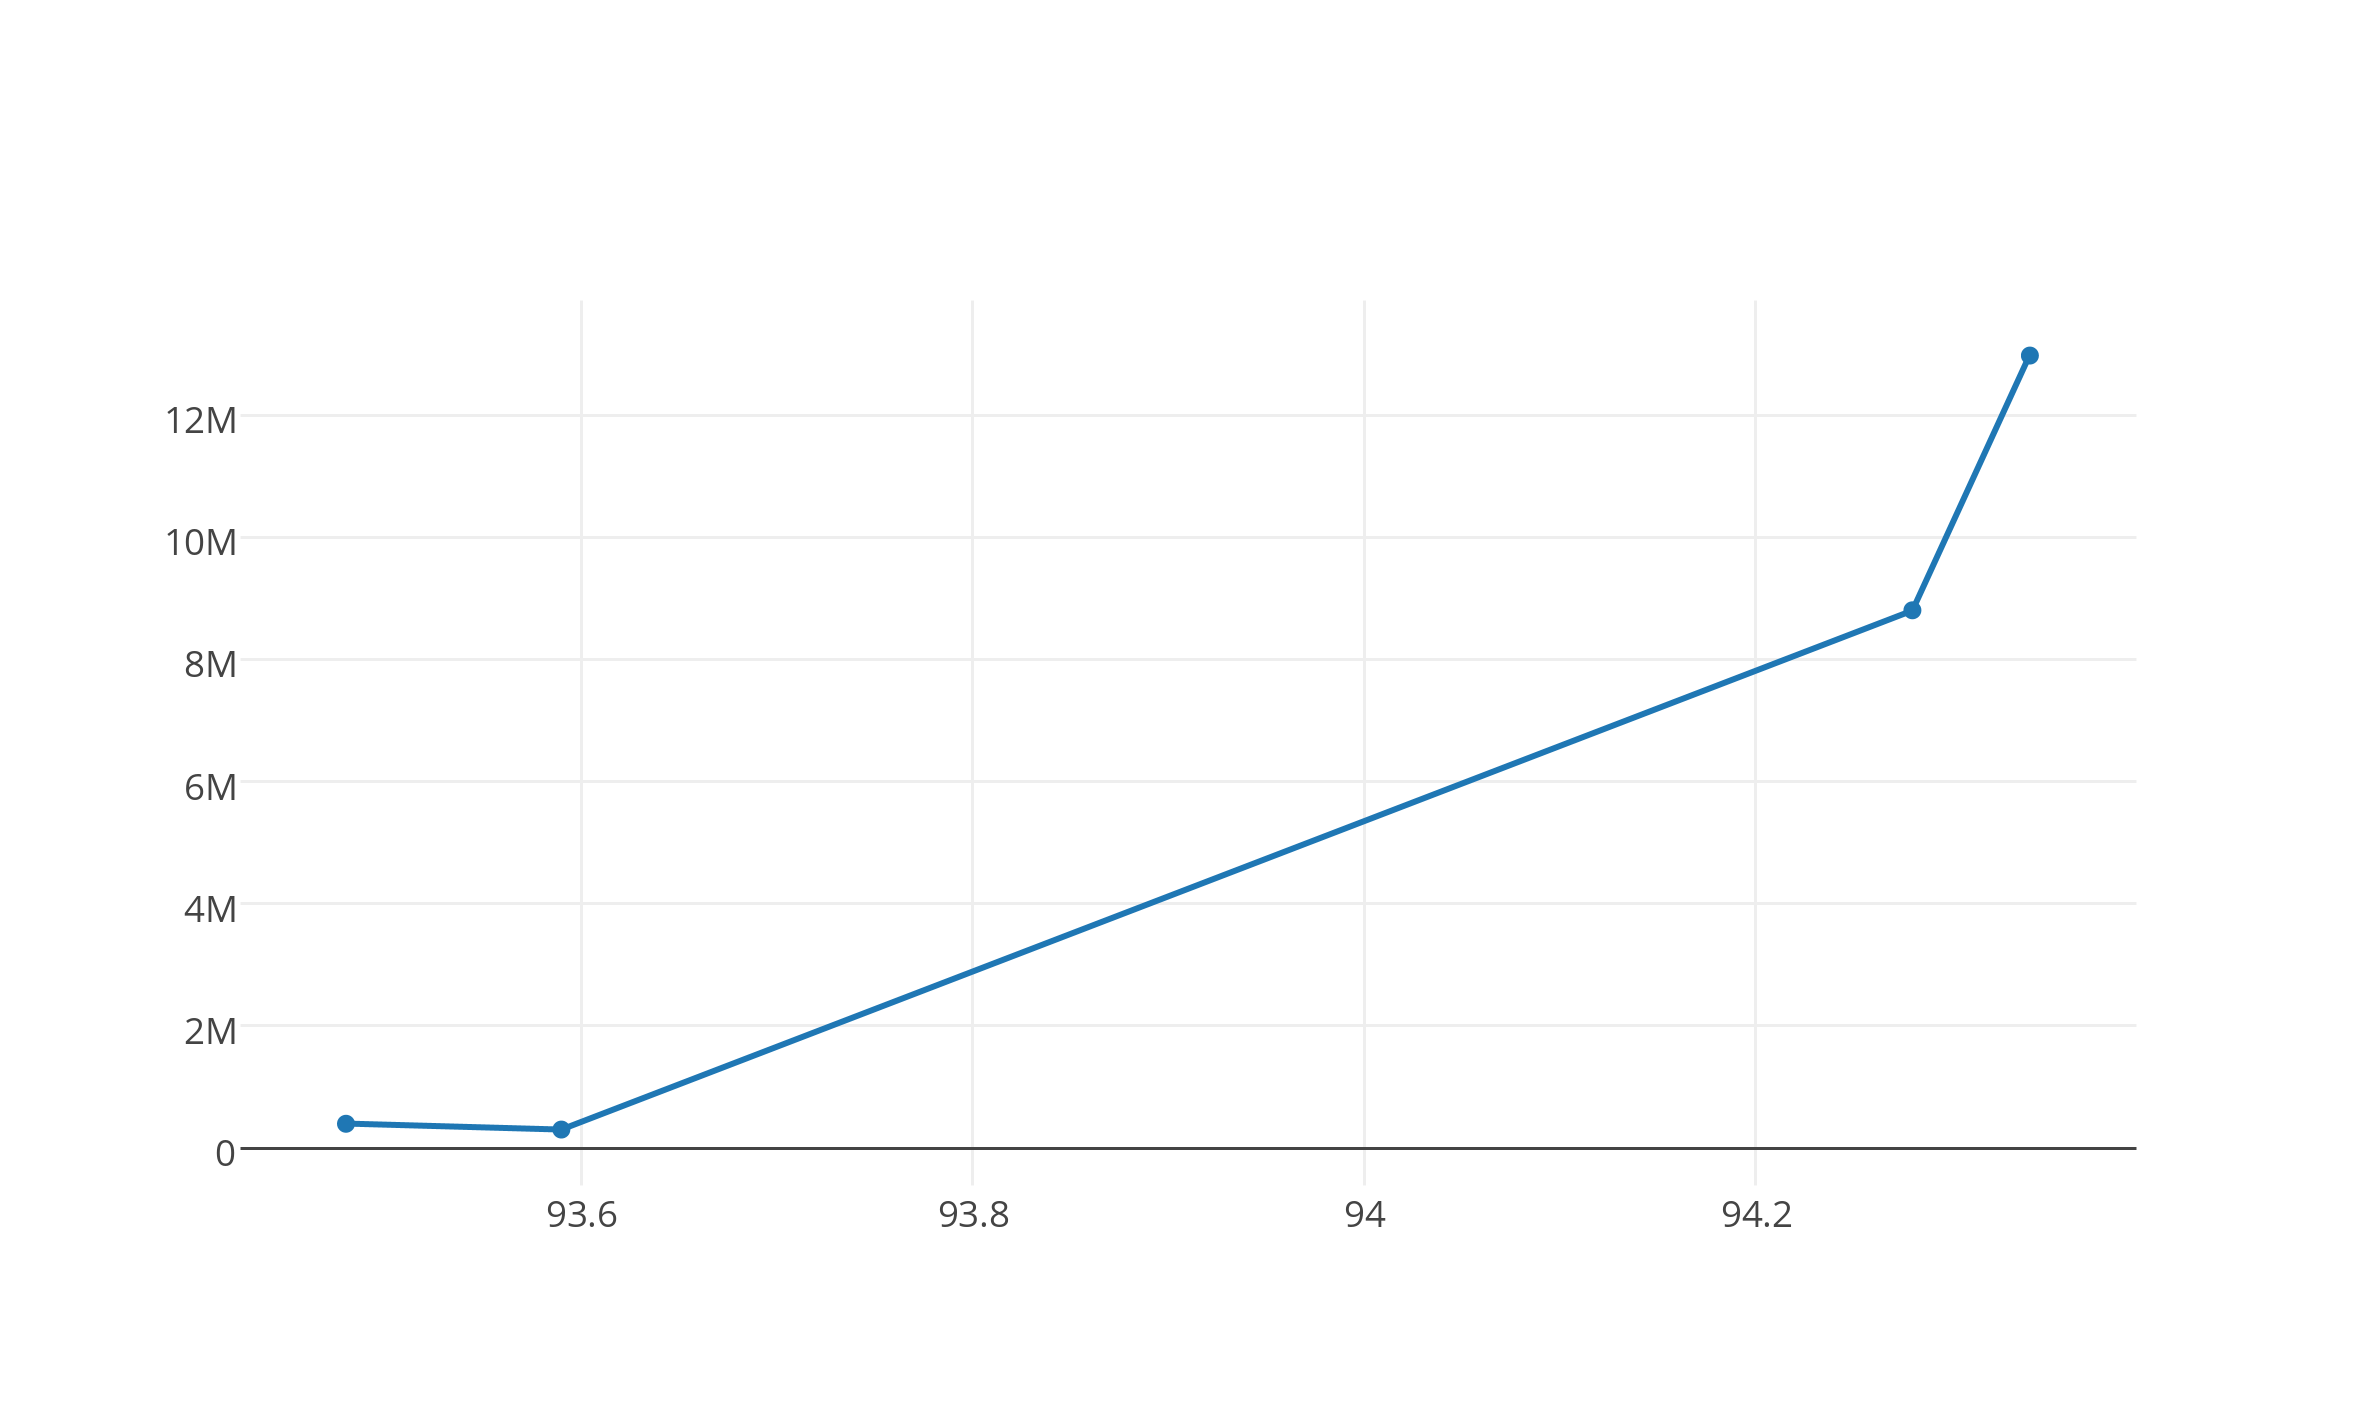
\includegraphics[scale=0.5]{res/crf_exp_num_features}
    \caption{The exponential increase of the number of features.}
    \label{fig:crf_exp_num_features}
\end{figure}

\chapter{Text classification with Na\"{\i}ve Bayes}

The goal of the text classification part is to predict labels starting from sentences. I trained a Na\"{\i}ve Bayes LM starting from..


Both the train\footnote{NLSPARQL.train.tok} and the test\footnote{NLSPARQL.test.tok} dataset has been modified before starting to train the LM. In fact, in both files multiple labels occur for some sentences. As a consequence, bad situations might occur as follows.
\begin{enumerate}
\item During the training, the probability of having \textbf{multiple labels} for same sentences has to be treated in a differant way.
\item During the test, the LM predicts only one label for each sentence. So it is necessary to \textbf{check} if the predicted label is in the set of the expected ones.
\end{enumerate}

\noindent
In order to solve both the previous problems, I considered sentences that are labelled by more than one label and I used a script which writes each sentence a number of times equal to the number of labels. Afterwards, I calculated the probability which can be expressed by the following expression.
\[ P(w_i | tag_j) = \frac{C(w_i | tag_j)}{C(w_i)} \]

\begin{table}[h!]
\small
	\begin{center}
	\begin{tabular}{|l|l|l|l|l|}
		\cline{2-5}
		\multicolumn{1}{r|}{} & accuracy & precision & recall & FB1 \\ \hline
		Simple & 72.42\% & 72.42\% & 72.42\% & 72.42 \\ \hline
	\end{tabular}
	\caption{Test results with Na\"{\i}ve Bayes.}
	\label{table:bayes_results}
	\end{center}
\end{table}



\chap{Conclusion}

This report has described the first project of the Language Understanding Systems course. It is focused on sequence labeling and text classification of a dataset which refers to the movie domain. The sequence labeling part has been computed in two ways using respectively two different tools: the first one was based on Finite State Transducers (FST) while the second one was based on Conditional Random Fields (CRF++). The text classification part has been done using Na\"{\i}ve Bayes with Maximum Likelihood. Different train techniques has been experimented and test results for each of these has been reported.

As result of the sequence labeling with FST, the high score I got is 94.13\% of accuracy and 92.87\% of precision. To reach these values I used a LM trained without lemmas and with a maximum n-gram order count equal to 4.

With CRF++ the highest score I reached is 94.34\% of accuracy and 86.13\% of precision (Template D). However, these values came with 12974573 features, which is very high respect to 8804873 features which allowd me to reach 94.28\% of accuracy and 84.79\% of precision (Template C).

\end{document}